\documentclass[]{article}%(fold)
\usepackage[utf8]{inputenc}
\usepackage{fullpage,ifpdf,url,authblk,xspace}
\renewcommand\Affilfont{\small}

\ifpdf
\usepackage[pdftex]{graphicx}
\else
\usepackage{graphicx}
\fi

%\date{}

\title{TV and the Social Web in the NoTube Project}

\author[1]{Libby Miller}
\author[2]{Dan Brickley}
\author[1]{Vicky Buser}
\author[1]{Yves Raimond}
\author[3]{Members of the NoTube project}

\affil[1]{BBC, UK}
\affil[2]{Vrije Universiteit, Amsterdam}
\affil[3]{http://notube.tv}


%(end)
\begin{document}


\ifpdf
\DeclareGraphicsExtensions{.pdf, .jpg, .tif}
\else
\DeclareGraphicsExtensions{.eps, .jpg}
\fi

\maketitle%(end)
% (fold)
\emph{This is a draft short version of the NoTube deliverable D7c.1. It may be updated in the future.}
\\
\\
Three principles:
\\
\\
\indent{{\bf Conversation is king: content is just something to talk about.\footnote{\url{http://www.boingboing.net/2006/10/10/disney-exec-piracy-i.html}}}}
\\
\\
\indent{{\bf The TV should be part of the Web, not a walled garden.}}
\\
\\
\indent{{\bf Connecting the TV to the Web doesn't have to mean showing the Web on the TV screen.} }
\\
\\
As part of the NoTube project we aim to show how these can be implemented using open APIs and formats, guided by practical scenarios, initially using a software media centre controlled by a handheld companion device. 

The result will be software, APIs and formats that can enable contributions to the `NoTube Network': a unified global network of annotations, ratings, comments, descriptions, related links and tags, attached to unique, re-referencable identifiers for programmes, segments, series, brands and channels, and that can provide new means for users to inform, educate and entertain themselves online. 

Crucial to success will be the open APIs, formats and protocols we we will use and create, so that the principles of an open, Web-connected TV can be applied to multiple environments, including watching on media centres, Web-based TV and mobile video.

\section{The NoTube Network}

Particular pieces of broadcast video content are not usually available to people in different geographical areas at the same time (generally they are at the mercy of various content-based agreements, scheduling times may be different, timezones different and so on). The same is true of many video on demand systems such as Hulu or Joost. 

Nevertheless people in different geographical areas can and (we believe) should be able to create annotations (`User Generated Content') against these programmes. That is, they should all be able to refer to the same thing even if they cannot or do not want to watch it all at the same time. 

Annotations could be as simple as `I watched this', or could be tags, reviews, ratings, or anything else people want to say about pieces of media content. While these kinds of functionalities are starting to exist in some isolated systems, the data is rarely made available through standard APIs and formats that allow users to take control of their information, or groups of users to make more social use of TV while using different systems.

Below we show a plan for how that data can be made useful and reuseable by connecting the TV to the Web more closely.

% (end)
\section*{Scenarios for Personalized TV and the Social Web} % (fold)

The NoTube project is based around three usecases. In this part of the NoTube Project, we will contribute to the `NoTube Network' guided by scenarios from one usecase (`TV and the Social Web'), showing how data might flow between the Web and the TV in both directions.

\subsection{Scenario 1: Recommendations on my TV based on my web behaviour}

Jana wants to see recommendations based on her social activity on her TV when she gets 
home at night. She talks a lot on twitter and facebook about what she watches in the context 
of her online social life, and so do her friends, and doesn't see why she should have to 
explicitly tell any system what her preferences are. She wants to see recommendations clearly 
featured on the user interface of her media centre. 

\subsection{Scenario 2: Do you want to know more?}

While watching on her TV Jana sometimes would like more information about a programme. 
She'd like to be able to mark a programme to come back to it later and find out more 
about it. She doesn't necessarily want to have her laptop open all the time during this and 
neither does she want to interfere with the playing of the programme too much as she often 
watches TV with other people in the same room. 

\subsection{Scenario 3: Add to playlist}

While at work, when he gets a link sent to him via Twitter or Facebook, Stephen would like to add programmes to his playlist on the media centre for watching later.

\subsection{The Scenarios and the `NoTube Network'}

These are scenarios that will only be of immediate relevance to a relatively unusual group of people at the current time: those who commonly watch TV on their media centre, and who watch a lot of on-demand media and who heavily use social networking sites. However it is possible to relate them to the majority of users as well, who are currently only consuming broadcast content.

In Scenario 2, \emph{wanting to know something more about a programme and remembering it for later} is the key idea, a desire common to many TV watchers, regardless of the technologies they use. In Scenario 1, \emph{filtering interesting programmes and bringing them to the user's attention} is the most important aspect, and one becoming increasingly relevant to all TV watchers as channels proliferate. In Scenario 3, \emph{saving items to watch later} is conceptually similar to recording programmes on video or DVD. Finally, using a setup that replicates at least the feeling of watching TV in a living room allows us to address the most common way of watching TV.
\\

{\bf The APIs and data formats - the components that allow us to make the prototype but also specifically allow us to filter an EPG, export activity feeds, control a television and so on - are the pieces that can be reused in other user situations and can form part of the `NoTube Network'.}

\section{Our Assumptions}

\subsection{Roughly Replicate the Traditional TV Watching Format}

Although TV-watching often takes place alone, nevertheless it is also a social activity, encompassing direct interaction with other individuals while either watching in the same place or separated by distance and communicating online. For the first prototypes we focus on cases where there may be someone else in the same room, and so the user doesn't necessarily want to change channel or otherwise disrupt the viewing experience on the TV screen.

\subsection{Conversation is King}

\emph{``Conversation is king. Content is just something to talk about.''}\footnote{\url{http://www.boingboing.net/2006/10/10/disney-exec-piracy-i.html}} Whether social activity is occurring online or offline it's a crucial part of TV, and once communication is online, there needs to be a way for people to refer to the content in emails, social networking sites, texts and so on. Therefore we require ways to refer accurately, uniquely and dereferencably to items of interest, including programmes, contributors, genres, series, brands.

\subsection{Connecting the TV to the Web doesn't have to mean showing the Web on the TV screen}

Flowing directly from the face-to-face social user assumption, especially coupled with the difficulties of data input commonly experienced with remote devices on a TV, comes the idea that the Web is a useful companion to TV rather than the Web being on the TV screen. Therefore in this first prototype we are interested in companion devices when watching the TV, used to access the web {\bf and} get information from the TV.

\subsection{The TV is Part of the Web, not a Walled Garden}

The third scenario illustrates this nicely: if the user sees something on the Web they can't watch now but are still interested to watch later when they have more time, then why should their TV not understand a link? Similarly, the plethora of APIs and protocols that underlie the modern Web and help users store their data at their convenience and where they get most benefit from it could also be applied to TV.

\section{Linked Data and TV}

In the project, we use Semantic Web\footnote{\url{http://www.w3.org/Talks/WWW94Tim/}} vocabularies and technologies where useful, particularly Linked Data. Linked Data is rather like putting multiple databases on the web and giving each item of interest a globally unique key that allows you to make links between different databases. In the Linked Data world, these keys are also dereferencable URLs, which can give more machine-readable information about themselves when fetched, such as what they are connected to, what sort of a thing they are and what properties or attributes they have. The items of interest can be anything - people, documents, places, pictures, videos, anything that can be identified. 

\subsection{Linked data and Content Filters}

Using Linked Data enables interesting links to be made between items in a partially automated way. For example by combining MusicBrainz with DBpedia, which is derived from Wikipedia, we may be able to find out that a piece of music is related in an interesting way to another piece of music. Some of the links between the two pieces of music might be very uninteresting (`both artists were American'), but we might find something interesting by linking up these datasets, (such as `both artists worked in Detroit in the 1960s'). This is a way to suggest content of interest to someone who has just listened to music by the first artist, or to provide more information of interest about the first artist (for example as part of the `Do you want to know more' scenario). The Music Bore\footnote{\url{http://www.bbc.co.uk/blogs/radiolabs/2009/07/the_music_bore.shtml}} and dbrec\footnote{\url{http://dbrec.net/}} are examples of using this technique without user profiles. 

We believe that a profile for a user stating that she is interested in particular things (such as a particular kind of music) will allow useful personalised content filters to be created, by narrowing the types of linked data connections that should be followed for this user. Further, if the user profile can state in a machine-processible fashion the preferences of the user over multiple interests in context then a smart linked data filter should be able to order the suggestions in priority of interestingness. 

One of the nice features of this approach is that cross-domain recommendations can be produced, for example a TV programme could be used to recommend related music, or related documents or books. Another useful feature is that this technique can provide contentful explanations of why the user might be interested in a piece of content, as opposed to the `black box' explanations of Amazon-style collaborative filtering techniques (e.g. `You might like Y because other people who bought X also bought Y').

One of the outputs of the NoTube project is planned to be research in applying complex profiles to linked data content filters of this kind. 

\subsection{User profiling from social activity data}

Many organisations gather data on individuals, for example supermarket clubcards, Web search engines, and broadcast organisations. They tend to be interested in people matching statistical trends that they can use to target advertising or products to specific individuals, and in particular to target people with items they actually want to purchase or use. Here we are interested in something similar: to suggest content to people that they are actually interested in. The means we have chosen is to harvest the data about individuals on the Web {\bf with their explicit consent} to create machine-readable profiles that they control. The part of NoTube implementing this is the `Beancounter', which enables users to securely add social networks they are members of to generate a profile and edit the result, so they get suggestions about the things they are interested in.

\subsection{BBC Programmes Linked Data}

As part of its website the BBC aims to produce a URL for each programme created, available in HTML and RDF formats, and linked to other items of interest, such as series, genre and contributors, using the BBC Programmes Ontology\footnote{\url{http://www.bbc.co.uk/ontologies/programmes/}} and in some cases MusicBrainz and DBpedia identifiers. In doing so it forms part of the Linked Data Cloud\footnote{\url{http://linkeddata.org/}}. This is separate to its iPlayer catchup service, although where video of the programme is available it will be linked from or embedded in the programme page.

This makes for a useful testbed for these ideas: without adding to the BBC data, we can easily create bookmarking systems, because there has a URL for most recent programmes - for the BBC, TV already links to the Web. In addition, because the BBC Programmes Ontology is an FRBR-based vocabulary, it distinguishes between items of interest at the `Brand' (e.g. Dr Who), `Series' (e.g. Dr Who Series 8), `Programme' (Dr Who Series 8, episode 5'), `Version'  (Dr Who Series 8, episode 5 with signing). It also describes when it was broadcast, the genre it is placed in. and in some cases who the contributors were. This means that extremely simple recommendations such as 'you might like this episode of Dr Who because you liked the series Dr Who Series 8' can be made using this data alone, using the identifiers and the broadcast schedule.

\subsection{Data Enhancement}

For more interesting and for non-BBC content suggestion and filtering there is substantial work to be done in 

\begin{itemize}
\item{Concept identification: creating new links between items of interest and other vocabularies, using natural language processing or ontology matching}
\item{Matching different identifiers for the same item. In the example of the database on the Web, where there are different unique keys coming form different databases which refer to the same thing, we need to find them and create links between them. An example might be a BBC programme URL for Murder She wrote, Series 12, episode 4 and the equivalent IMDB URL.}
\item{Matching of schedule and TVAnytime broadcast identifiers and Web programme identifiers}
\item{Matching user channel or programme availability to any given user, for example using schedule data and location data} 
\end{itemize}

while for the bookmarking and more information scenarios, there is a need for

\begin{itemize}
\item{Generated or existing URLs for channels and programmes}
\end{itemize}

\section{Architecture}

\begin{figure}[htbp]
\begin{center}
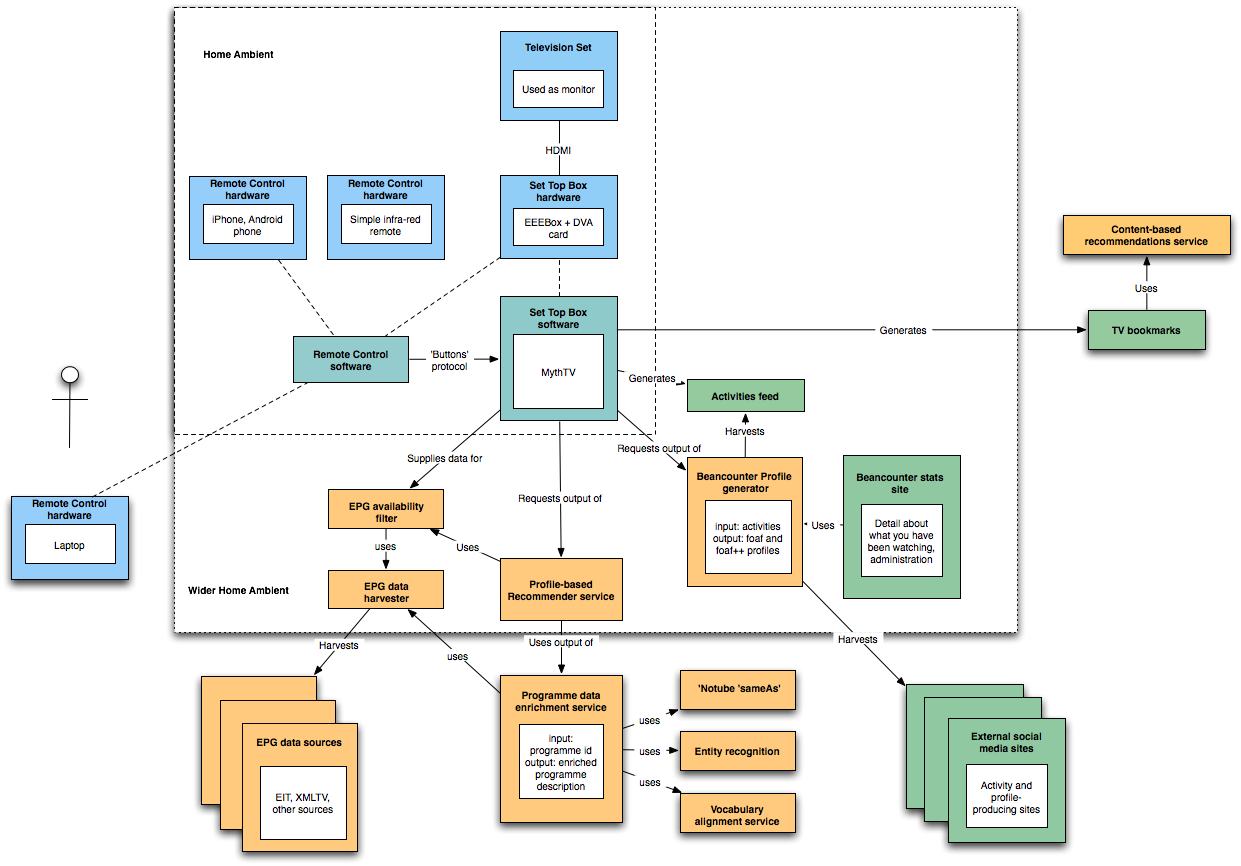
\includegraphics[width=7in]{architecture.png}
\caption{Architecture} \label{fig:architecture}
\end{center}
\end{figure}

The architecture is comprised of a set of services called by a sophisticated software media centre authorised by credentials sent from a smart phone acting as a remote control.

The user's remote `companion' device enables secure identification of the user to the media centre, which then can pass credentials from the device to other services such as the Beancounter and the recommender, which in turn use the various enhancement services.

It will be possible to run the beancounter and simple recommenders inside the home ambient for enhanced security and privacy, as the detailed architectural diagram Figure \ref{fig:architecture} shows.

\subsection{Scenario 1: Recommendations for me on my TV based on my web behaviour}

This scenario requires that the user pre-register on the Beancounter profiler, adding one or more sources of data from existing social media sites that she uses. When she comes home to her TV and media centre, she can view recommendations based on her Beancounter profile within the TV's programme guide (EPG), operating the media centre with her iPhone acting as a remote control. Profile access and recommendations for a given profile are via RESTful APIs, with security (if required) planned to be handled by OAuth.\footnote{\url{http://oauth.net/}}

Very important here for recommendations is the availability of programmes to the user. Broadcast content in particular is usually restricted to a particular geographical area, and some Web-based services like Hulu and iPlayer also restrict their content geographically. Similarly broadcast content is restricted by time (although there may be repeats) and some Web-based services also limit availability to a short period of time. A recommendations service must only recommend content available to the user.

Also important is the identification of channels and programmes to the user from the recommender to their media centre. Multiple formal and informal names for channels and programmes are used and a service to combine these is required (more in Scenario 3 below).


\subsection{Scenario 2: Do you want to know more?}

Scenario 2 is about finding more information automatically about a particular programme. Here we make use of the capabilities of the companion device to allow Jana to find out more information without disturbing anyone else in the room. An automated, linked-data service (which may include data enhancement services) can be employed to suggest interesting and novel information about a programme; if this is not available then basic data can be provided from a local or remote programmes data store.

Data enhancement services could include entity recognition for finding commonly used URLs for programmes, and `same as' functionality for linking various URLs about the same entity from across the linked data cloud. For example `Doctor Who' has the RDF (linked data) URL of \url{http://www.bbc.co.uk/programmes/b006q2x0.rdf}, in DBdedia it is \url{http://dbpedia.org/data/Doctor_Who.rdf}, in Freebase \footnote{\url{http://www.freebase.com/}} it is \url{http://rdf.freebase.com/rdf/en.doctor_who} and in IMDB (not part of the linked data cloud but commonly used to refer to Film and TV entities) it is \url{http://www.imdb.com/title/tt0436992/}. 

An additional part of the problem is very similar to the linked data recommendations issue referred to above: finding {\bf interesting} items through a cloud of links requires some filtering; this is important an area of research for the project.

Architecturally, we have chosen to link the media centre with the remote using the XMPP `buttons' protocol, where the media centre has its own XMPP-addressible unique identifier which has the notion of trusted contacts. This potentially solves some of the security and privacy issues raised in scenario 3 and in more detail below. 


\subsection{Scenario 3: Add to media centre's `to watch' list, while away from Local Area Network}

In Scenario 3, the user receives news of interesting media in of a context when he cannot easily watch it. The most obvious example is via social media, where the user's friends may tell him about programmes of interest that he cannot or does not want to consume immediately but might be interested to watch when he is more comfortable at home. These social networking news items are often transient and so remembering for later is useful. They commonly use Web URLs as a means to describe programmes, although sometimes shorthand names for TV channels or just the titles of programmes may be used. This scenario is particularly relevant to long-form content rather than short pieces of video.

This functionality requires well-defined APIs connecting the media centre within the `home ambient' and the wider network, together with appropriate authentication and security mechanisms to prevent unauthorised high-resource-consumption downloads. 

It also requires well-defined descriptors for programmes and channels which are usable and accessible on the Web {\bf and} from a media centre. In some cases a url is sufficient for both of these but in other cases there need to be mappings made between formal names (e.g. DVB 'CRIDs' or BBC programmes or iPlayer URIs), informal names (often as `tags') and persistent or transitory URLs for programmes and channels. There may also be a need for services that can be used to determine what was on at a particular time on a particular channel, title resolvers and other data enhancement services that enable reference to the same item of interest.



\section{Tasks and Implementation}

The prototype implementation will use a companion device (an iPhone in this case) to control a software media centre (MythTV) and also receive information from the media centre to allow the user to plan viewing without disturbing others (e.g. by browsing available programmes on the device). The user can also find out more information about a programme using the device, or access existing social networks from it in order to talk about the programme.

We are currently at the proof-of-concept stage of implementation.

\subsection{Scenario 1: View Recommendations in an EPG}

The screenshots in Figures \ref{fig:mythtv-recommendations} and \ref{fig:mythweb-recommendations} show recommendations appearing as a changed UI in MythTV frontend media centre and its web-based navigator. This shows that the UI can be altered, and in building it we discovered the fields we needed for the output of the recommendations engine: a consistent channel identifier and an exact date-time value.

\begin{figure}[htbp]
\begin{center}
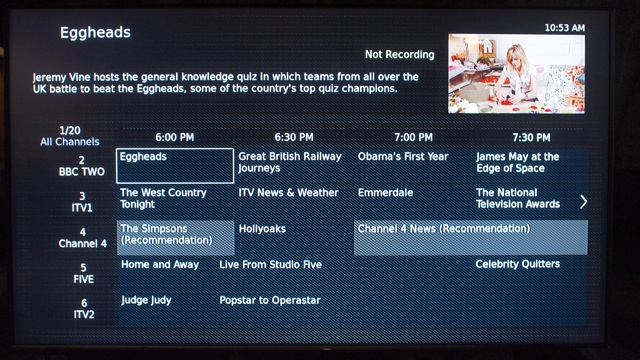
\includegraphics[width=6in]{mythtv-recommendations.jpg}
\caption{Recommendations appearing in MythTV frontend EPG} \label{fig:mythtv-recommendations}
\end{center}
\end{figure}

\begin{figure}[htbp]
\begin{center}
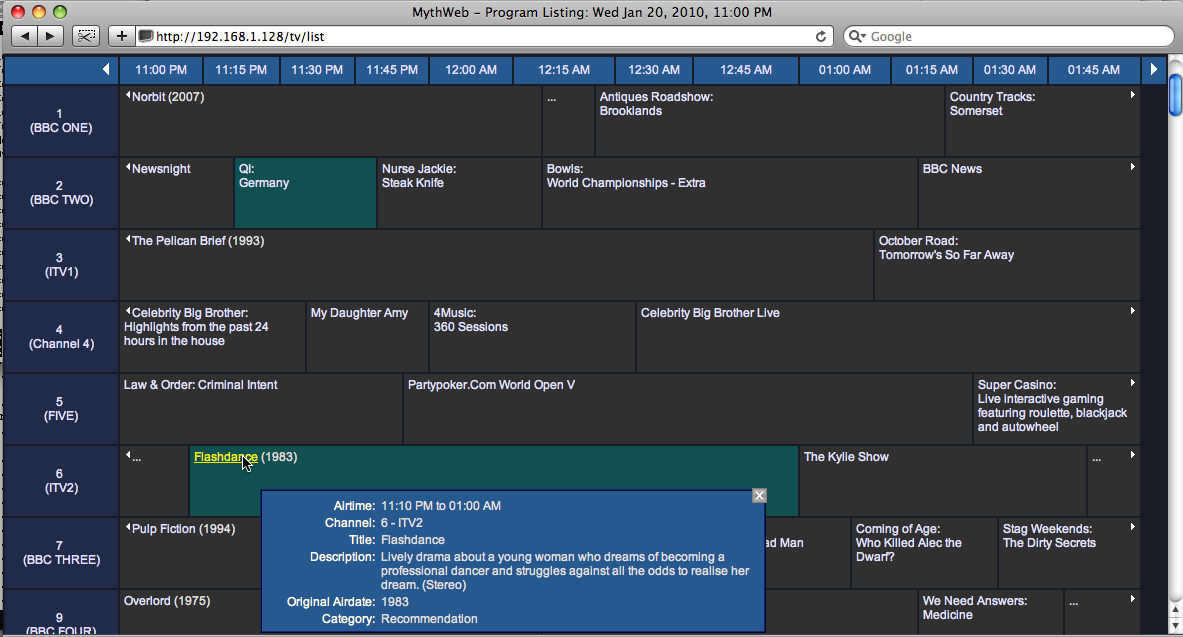
\includegraphics[width=6in]{mythweb-screen.png}
\caption{Recommendations appearing in MythTV web frontend (MythWeb)} \label{fig:mythweb-recommendations}
\end{center}
\end{figure}


\subsection{Scenario 2: Bookmark and Tag a Programme from TV to the Web}

The screenshots in Figures \ref{fig:bot} and \ref{fig:bookmarks} show our proof-of-concept where we used a text-based XMPP interface via MythTV to create bookmarks in the bookmarking site delicious.com. XMPP is used where http would also work because we want to explore XMPPs built-in `friending' mechanism in later iterations for security and privacy. The user would not be expected to type the commands in manually in the finished interface.

\subsection{Future Work}

The implementation is ongoing, and we hope to show functioning and usable implementations of all three scenarios by May 2010. Later we will place particular emphasis on its {\bf security} and {\bf privacy} aspects. In particular:

\begin{itemize}
\item{Securely pairing devices to media centres}
\item{Securely accessing 	private data from social networking sites}
\item{User experience of privacy in the Beancounter and elsewhere}
\end{itemize}


\begin{figure}[htbp]
\begin{center}
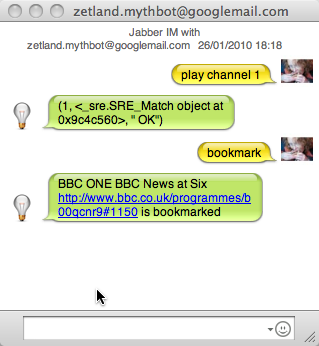
\includegraphics[width=3in]{bot.png}
\caption{Jabber bot communication with MythTV and Delicious} \label{fig:bot}
\end{center}
\end{figure}

\begin{figure}[htbp]
\begin{center}
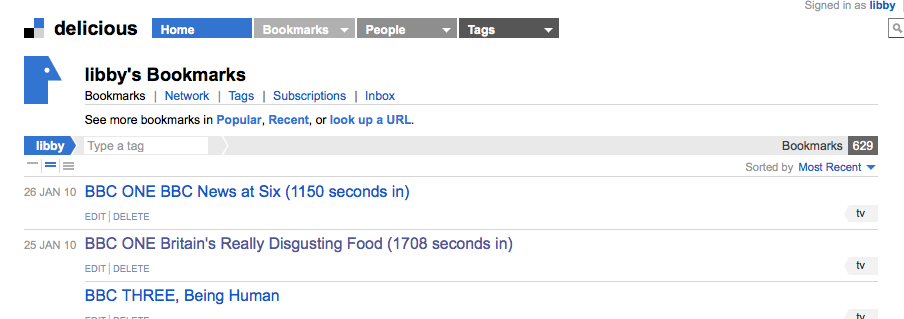
\includegraphics[width=6in]{bookmarks.png}
\caption{TV bookmarks appearing in Delicious} \label{fig:bookmarks}
\end{center}
\end{figure}


\end{document}
